\section{NP-completeness of the Min Cut-Path Problem}
\label{sec:np-completeness}
In this section, we show that the decision version of the \MinCutPath{} problem is NP-complete.
Our proof proceeds via a sequence of polynomial-time reductions.
We begin with the well-known \ThreeSAT{} problem, which is formally defined as follows.





\begin{problem}[\ThreeSAT]
Let $U = \{x_1, x_2, \dots, x_n\}$ be a finite set of Boolean variables, and let
$\mathcal{C} = \{C_1, C_2, \dots, C_m\}$ be a collection of clauses, where each clause
$C_k$ is a disjunction of exactly three literals, and each literal is either a variable $x_i$ or its negation $\neg x_i$.

The \ThreeSAT{} decision problem is defined as follows:

\begin{center}
\begin{tabular}{p{0.12\linewidth}p{0.8\linewidth}}
\textbf{Input:} & A finite set of Boolean variables $U$ and a collection $\mathcal{C}$ of clauses, each containing exactly three literals.\\
\textbf{Question:} & Does there exist a truth assignment $\tau: U \rightarrow \{\mathsf{true}, \mathsf{false}\}$ such that every clause $C_k \in \mathcal{C}$ evaluates to \textsf{true} under $\tau$?
\end{tabular}
\end{center}
\end{problem}


It is well known that \ThreeSAT{} is NP-complete~\cite{Cook1971Complexity}.
Throughout this section, $n$ and $m$ denote the numbers of variables and clauses of the \ThreeSAT{} instance under consideration.

Our approach is based on a two-step reduction.
Instead of reducing \ThreeSAT{} to \MinCutPath{} directly, we introduce an intermediate problem, the \SSP{} problem.
First, we show that this problem is NP-complete by a polynomial-time reduction from \ThreeSAT{} (Section~\ref{sec:ssp}).
Second, we reduce \SSP{} to \MinCutPath{} (Section~\ref{sec:ssp-to-mcp}).


\subsection{The Separating Shortest Path Problem}\label{sec:ssp}
In contrast to the \MinCutPath{} problem, where the objective is to find a set of edges that simultaneously contains both a $u$--$v$ path and a $u$--$v$ cut, the \SSP{} problem focuses solely on identifying a shortest path with a specific separation property.
Namely, we ask whether, among all shortest $u$--$v$ paths in the graph, there exists one whose removal disconnects $u$ and $v$.

\begin{problem}[\SSP]
Let $G = (V,E)$ be an undirected graph and let $u,v \in V$ be two distinct vertices.
A shortest $u$--$v$ path $P$ is called a \emph{separating shortest path} if the graph $G \setminus P$ contains no $u$--$v$ path.
The \SSP{} decision problem is defined as follows:

\begin{center}
\begin{tabular}{p{0.12\linewidth}p{0.8\linewidth}}
\textbf{Input:} & A graph $G = (V,E)$ and two distinct vertices $u,v \in V$.\\
\textbf{Question:} & Does there exist a shortest $u$--$v$ path in $G$ that is a separating shortest path?
\end{tabular}
\end{center}
\end{problem}

Note that, unlike \MinCutPath, the \SSP{} problem is not an optimization problem; it merely asks for the existence of a shortest path with a certain property.
This distinction allows us to construct a more direct reduction from \ThreeSAT.




\subsubsection{Gadgets and Basic Operations for the Reduction}

To establish the NP-completeness of \SSP, we introduce a collection of \emph{gadgets} and \emph{basic operations} on them.
These gadgets and operations are the elementary building blocks of our reduction from \ThreeSAT{} to \SSP.
They allow us to represent the logical structure of a formula within a graph in a modular way.

The construction consists of two parts:
\begin{enumerate}
    \item the \emph{base structure}, also referred to as the \emph{chain};
    \item the \emph{threads}, which are threaded through the base structure.
\end{enumerate}

Figure~\ref{fig:chain-threads} gives a schematic overview of the two types of gadgets and of the layout of the construction.


\begin{figure}[H]
    \centering
    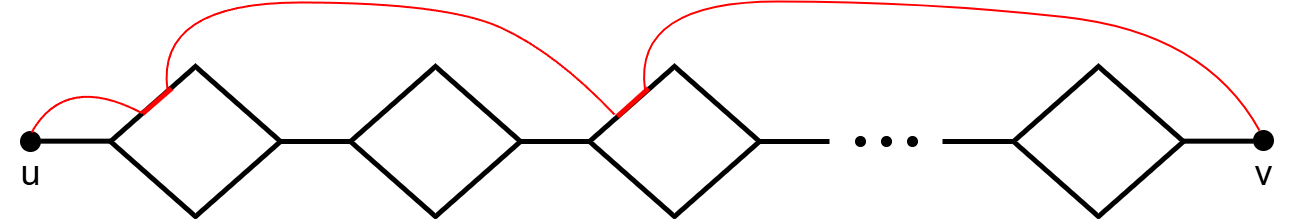
\includegraphics[width=145mm]{img/chain-threads.png}
    \caption{Layout of the construction: the chain (black) and a thread (red)}
    \label{fig:chain-threads}
\end{figure}
We now present the individual gadgets and operations in detail.


\paragraph{Chain.}
We begin with the smallest component among the gadgets, the \emph{chain link}.
It is a cycle with two distinguished vertices $p$ and $q$ that split it into two paths of equal length.


\begin{definition}[Chain Link]
\label{def:chain-link}
Let $G=(V,E)$ be a graph and let $p,q \in V$ be two distinct vertices.
A \emph{$(p,q)$-chain link} is a subgraph $L \subseteq G$ such that:
\begin{enumerate}
    \item $L$ is a simple cycle in $G$;
    \item the vertices $p$ and $q$ lie on $L$ and partition it into two internally disjoint $p$--$q$ paths;
    \item these two $p$--$q$ paths have equal length.
\end{enumerate}
We refer to one of the two $p$--$q$ paths as the \emph{positive path} of the chain link and to the other as the \emph{negative path}.
When a chain link is used inside a chain, its boundary vertices are exactly $p$ and~$q$, i.e., the points where the adjacent single edges of the chain are attached.
\end{definition}


\begin{figure}[H]
    \centering
    
\includegraphics[width=50mm]{img/chain-link.png}
    \caption{A chain link}
    \label{fig:chain-link}
\end{figure}



The chain forms the backbone of the construction.
Its defining feature is the strict alternation between single edges and chain links.
The structure always begins with a single edge, continues with a chain link, then again with a single edge, and so on, and it finally ends with a single edge.
Formally:

\begin{definition}[Chain]
\label{def:chain}
Let $G=(V,E)$ be a graph, and let $u,v\in V$.
We say that $G$ is a \emph{$u$--$v$ chain} with $r$ chain links if it is the union of edge-disjoint subgraphs
\[
G = H_1 \cup L_1 \cup H_2 \cup L_2 \cup \cdots \cup L_r \cup H_{r+1},
\]
where:
\begin{enumerate}
    \item each $H_i$ consists of a single edge with end-vertices $p_i,q_i$;
    \item each $L_i$ is a $(q_i,p_{i+1})$-chain link;
    \item the first end-vertex $p_1$ coincides with $u$ and the last end-vertex $q_{r+1}$ coincides with $v$;
    \item two of these subgraphs share a vertex only if they are consecutive, and then they share exactly one vertex ($q_i$ or $p_{i+1}$).
\end{enumerate}
Every $u$--$v$ path in a chain traverses all single edges and, in each chain link, either its positive or its negative path.
\end{definition}

\begin{figure}[H]
    \centering
    
\includegraphics[width=145mm]{img/chain.png}
    \caption{A chain}
    \label{fig:chain}
\end{figure}



In the reduction from \ThreeSAT{} to \SSP, chain links have specific roles that reflect the structure of clauses and variables.
Let $C_1, C_2, \dots, C_m$ denote the clauses of the input formula and let $x_1, x_2, \dots, x_n$ denote its variables.
Each chain link is assigned to exactly one of the following three types:

\begin{enumerate}
    \item \textbf{Initialization chain link.}
    For each variable $x_i$ we introduce an initialization chain link, denoted $I_i$.
    This link marks the beginning of the part of the chain that corresponds to the variable $x_i$. The total number of initialization chain links is $n$.

    \item \textbf{Terminal chain link.}
    For each variable $x_i$ we also introduce a terminal chain link, denoted $T_i$.
    This link marks the end of the part of the chain associated with the variable $x_i$. The total number of terminal chain links is $n$.

    \item \textbf{Literal chain link.}
    For each clause $C_k = (\ell_1 \vee \ell_2 \vee \ell_3)$ and each $j \in \{1,2,3\}$, let $x_i$ be the variable of the literal $\ell_j$.
    We introduce a literal chain link, denoted $L_{j,k,i}$ (or $L_{j,k}$ for short).
    This link represents the occurrence of the variable $x_i$ as the $j$-th literal of the clause $C_k$.
    The total number of literal chain links is $3m$.

\end{enumerate}

The chain links that belong to one variable are consecutive in the chain, as illustrated in Figure~\ref{fig:chain-link-types}.

\begin{figure}[H]
    \centering
    
\includegraphics[width=145mm]{img/chain-link-types.png}
    \caption{Chain links of a variable $x_i$: the initialization link, the literal links, and the terminal link}
    \label{fig:chain-link-types}
\end{figure}

In total, the construction contains exactly $3m + 2n$ chain links, accounting for all initialization, terminal, and literal links.

\paragraph{Threads and threading.}
Having defined the chain and its links, we now introduce the notion of \emph{threads}, which are paths that pass through the chain links.
The operation of inserting such paths into the chain is called \emph{threading}. More precisely:

\begin{definition}[Thread]
\label{def:thread}
Let $G=(V,E)$ be a graph containing a $u$--$v$ chain with chain links $L_1,L_2,\dots,L_r$.
A \emph{thread} is a $u$--$v$ path $P$ in $G$ such that:
\begin{enumerate}
    \item for each chain link $L_i$, the path $P$ shares at most one edge with $L_i$, and $P$ contains none of the single edges of the chain;
    \item $P$ is edge-disjoint from every other thread and shares only the vertices $u$ and $v$ with it.
\end{enumerate}
\end{definition}

Thus, threads can be seen as edge-disjoint $u$--$v$ paths that ``pass through'' the sequence of chain links, each touching a link in at most one edge.

Threads interact with chain links through the operation of \emph{threading}.
Intuitively, threading takes an edge of a chain link that has not yet been traversed by any existing thread, subdivides it into three consecutive edges, and then uses the middle edge as the unique crossing edge of the thread through that chain link.
Formally:

\begin{definition}[Threading]
\label{def:threading}
Let $L$ be a chain link in a $u$--$v$ chain, and let $P$ be a thread not yet passing through $L$.
The \emph{threading operation} on $(P,L)$ consists of the following elementary steps:
\begin{enumerate}
    \item Select an edge $e=\{x,y\}$ of $L$ that is not used by any existing thread.
    \item Subdivide $e$ into a path $x$--$z_1$--$z_2$--$y$ of three edges, introducing two new vertices $z_1,z_2$.
    \item Extend $P$ so that it traverses the middle edge $\{z_1,z_2\}$, called the \emph{crossing edge}, as its unique crossing of the chain link $L$.
\end{enumerate}
If the selected edge $e$ belongs to the positive path of $L$, we say that $P$ is \emph{positively threaded through $L$}; if $e$ belongs to the negative path of $L$, we say that $P$ is \emph{negatively threaded through $L$}.
In general, we say that the thread $P$ is \emph{threaded through $L$ at the edge $e$}.
\end{definition}

\begin{figure}[H]
    \centering
    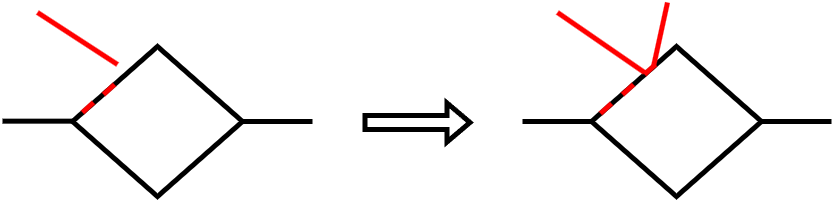
\includegraphics[width=145mm]{img/threading.png}
    \caption{The threading operation}
    \label{fig:threading}
\end{figure}


To capture the logical structure of the \ThreeSAT{} formula, each thread is assigned a specific role.
We distinguish three types of threads:

\begin{enumerate}
    \item \textbf{2-synchronization thread.}
    This thread passes through an initialization chain link $I_i$ and the corresponding terminal chain link $T_i$.
    Its purpose is to enforce synchronization, ensuring that every separating shortest path traverses either the positive paths or the negative paths in both $I_i$ and $T_i$.

    \item \textbf{3-synchronization thread.}
    This thread passes through the initialization chain link $I_i$, a literal chain link $L_{j,k,i}$, and the terminal chain link $T_i$ corresponding to the same variable $x_i$.
    Its role is to synchronize the traversal of the literal chain link with that of the initialization and terminal links of the variable $x_i$.

    \item \textbf{Clause thread.}
    For each clause $C_k = (\ell_{1} \vee \ell_{2} \vee \ell_{3})$, a clause thread is introduced that passes through the three literal chain links $L_{1,k}$, $L_{2,k}$, $L_{3,k}$ corresponding to $\ell_{1}, \ell_{2}, \ell_{3}$.
    This construction simulates the satisfaction requirement of the clause: for a separating shortest path to exist, at least one of the three literals must be satisfied.
\end{enumerate}

\subsubsection{NP-completeness of \textsc{Separating Shortest Path}}
We now prove that \SSP{} is NP-complete by a polynomial-time reduction from \ThreeSAT.
The reduction is constructive and relies on the chain and threading gadgets introduced above.
Before presenting the full construction, we introduce a few auxiliary procedures and notational conventions that allow us to describe the reduction precisely and concisely.

\paragraph{Auxiliary procedures.}
The reduction uses the following auxiliary procedures:
\begin{itemize}
    \item $\textsc{BuildChain}(u,v,r)$: constructs a $u$--$v$ chain with $r$ chain links, where each chain link is realized as a $4$-cycle.
    \item $\textsc{Thread}(u,v,[(K_1,\sigma_1),\dots,(K_t,\sigma_t)])$: creates a new thread from $u$ to $v$ that passes through the chain links $K_1,\dots,K_t$ in this order, where $\sigma_i \in \{+,-\}$ specifies whether the thread is threaded through $K_i$ positively or negatively.
    The $t$ crossing edges are joined to each other and to the vertices $u$ and $v$ by $t+1$ new, internally vertex-disjoint paths, which we call the \emph{connecting paths} of the thread.
    \item $\textsc{Calibrate}(G)$: equalizes the lengths of the relevant paths in two steps.
    First, in every chain link whose positive and negative paths have different lengths, an edge of the shorter path that is not a crossing edge is subdivided repeatedly until both paths have the same length.
    Second, let $\Lambda$ denote the number of edges of a $u$--$v$ path in the resulting chain; every connecting path of every thread is subdivided until it has at least $\Lambda$ edges.
\end{itemize}

\paragraph{Auxiliary notation.}
We also introduce the following notational conventions:
\begin{itemize}
    \item Occurrences: for each variable $x_i$, we denote by $O_i$ the set of all pairs $(j,k)$ such that the $j$-th literal of the clause $C_k$ is $x_i$ or $\neg x_i$.
    \item Sign function: for each literal $\ell$ we define
\[
s(\ell) =
\begin{cases}
+ & \text{if $\ell = x_i$ for some variable $x_i$,}\\
- & \text{if $\ell = \neg x_i$ for some variable $x_i$.}
\end{cases}
\]
\end{itemize}

\begin{theorem}
\label{thm:ssp-np-complete}
The \SSP{} problem is NP-complete.
\end{theorem}

\begin{proof}
We first describe the reduction, then prove its correctness, and finally bound its running time and show that the problem belongs to NP.

\paragraph{Reduction from 3-SAT.}
Given an instance of \ThreeSAT, we describe how to construct a graph $G$ with two distinguished vertices $u,v$ such that $G$ contains a separating shortest $u$--$v$ path if and only if the given formula is satisfiable.
The construction is summarized in Algorithm~\ref{alg:reduction}.


\begin{algorithm}[H]
\caption{Reduction from \ThreeSAT{} to \SSP}
\label{alg:reduction}
\begin{algorithmic}[1]
\Require Variables $U=\{x_1,\dots,x_n\}$, clauses $\mathcal{C}=\{C_1,\dots,C_m\}$
\Ensure Graph $G$, vertices $u,v$
\State $G \gets \textsc{BuildChain}(u,v,2n+3m)$
\For{$i \gets 1$ to $n$}
    \State reserve the next $2+|O_i|$ free chain links
    \State label the first of them as $I_i$ and the last of them as $T_i$
    \For{each $(j,k) \in O_i$}
        \State label the next free reserved link as $L_{j,k,i}$
    \EndFor
\EndFor
\For{$i \gets 1$ to $n$}
    \State $\textsc{Thread}(u,v,[(I_i,+),(T_i,-)])$
    \State $\textsc{Thread}(u,v,[(I_i,-),(T_i,+)])$
    \For{each $(j,k) \in O_i$}
        \State $\textsc{Thread}(u,v,[(I_i,+),(L_{j,k,i},-),(T_i,+)])$
        \State $\textsc{Thread}(u,v,[(I_i,-),(L_{j,k,i},+),(T_i,-)])$
    \EndFor
\EndFor
\For{$k \gets 1$ to $m$}
    \State $\ell_1,\ell_2,\ell_3 \gets$ the literals of $C_k$
    \State $\textsc{Thread}(u,v,[(L_{1,k},s(\ell_1)),(L_{2,k},s(\ell_2)),(L_{3,k},s(\ell_3))])$
\EndFor
\State $\textsc{Calibrate}(G)$
\State \Return $G$, $u$, $v$
\end{algorithmic}
\end{algorithm}

In words, the chain consists of $n$ consecutive blocks, one for each variable; the block of $x_i$ starts with $I_i$, ends with $T_i$, and contains the literal chain links of all occurrences of $x_i$ in between.
Each variable receives a pair of 2-synchronization threads, each occurrence of a variable receives a pair of 3-synchronization threads, and each clause receives one clause thread.
The final calibration step guarantees that both paths of every chain link have the same length and that the connecting paths of the threads are sufficiently long.

\paragraph{Correctness.}
We now show that the constructed instance of \SSP{} is equivalent to the original \ThreeSAT{} instance.
We call the $u$--$v$ paths of the chain \emph{chain paths}; a chain path is determined by choosing, in every chain link, either its positive or its negative path.
We say that a chain path $P$ \emph{hits} a thread if $P$ and the thread share an edge.
Since a thread shares only its crossing edges with the chain, a chain path $P$ hits a thread created by $\textsc{Thread}(u,v,[(K_1,\sigma_1),\dots,(K_t,\sigma_t)])$ if and only if, for some $i$, the path $P$ traverses the path of $K_i$ with the sign $\sigma_i$.

\paragraph{Shortest paths.}
After the calibration, all chain paths have the same length $\Lambda$.
Every other $u$--$v$ path $Q$ in $G$ contains an edge of some connecting path.
Since the internal vertices of a connecting path have degree two, $Q$ contains the whole connecting path, which has at least $\Lambda$ edges, and at least one further edge, because no connecting path joins $u$ and $v$ directly.
Hence $|Q| > \Lambda$, and the shortest $u$--$v$ paths in $G$ are exactly the chain paths.

\paragraph{Synchronization of variable gadgets.}
Every thread is a $u$--$v$ path. Therefore, a chain path $P$ can be separating only if it hits every thread.
\begin{itemize}
    \item \emph{2-synchronization threads:} the chain path $P$ hits both 2-synchronization threads of the variable $x_i$ if and only if it traverses paths of the same sign in $I_i$ and in $T_i$.
    Indeed, the first thread requires the positive path in $I_i$ or the negative path in $T_i$, and the second thread requires the negative path in $I_i$ or the positive path in $T_i$.
    \item \emph{3-synchronization threads:} if $P$ traverses paths of the same sign in $I_i$ and $T_i$, then it hits both 3-synchronization threads of a literal link $L_{j,k,i}$ if and only if it traverses the path of this sign in $L_{j,k,i}$ as well.
    Indeed, one of the two threads is hit exactly when $P$ uses the positive path in $I_i$ or $T_i$ or the negative path in $L_{j,k,i}$, and the other one exactly when $P$ uses the negative path in $I_i$ or $T_i$ or the positive path in $L_{j,k,i}$.
\end{itemize}
Consequently, a chain path hits all synchronization threads if and only if, for every variable $x_i$, it traverses paths of the same sign in all chain links of the block of $x_i$.
We call such a chain path \emph{consistent}.
Consistent chain paths correspond to truth assignments: we set $\tau(x_i)=\mathsf{true}$ if the path traverses the positive paths in the block of $x_i$, and $\tau(x_i)=\mathsf{false}$ otherwise.

\paragraph{Clause threads.}
Let $P$ be a consistent chain path with the truth assignment $\tau$, and let $C_k = (\ell_1 \vee \ell_2 \vee \ell_3)$ be a clause.
The path $P$ hits the clause thread of $C_k$ if and only if, for some $j$, it traverses the path of $L_{j,k}$ with the sign $s(\ell_j)$, i.e., if and only if $\tau$ satisfies the literal $\ell_j$.
Thus a consistent chain path hits all clause threads if and only if its truth assignment satisfies every clause.

\paragraph{Two-way correspondence.}
We complete the proof by establishing the equivalence:
\begin{enumerate}[label=(\alph*)]
    \item If there exists a separating shortest path $P$ in $G$, then one can extract a satisfying assignment for the original \ThreeSAT{} instance.

    Since $P$ is a shortest $u$--$v$ path, it is a chain path, and since it is separating, it hits every thread.
    By the synchronization property, $P$ is consistent, so it determines a truth assignment $\tau$.
    Moreover, $P$ hits every clause thread, which means that $\tau$ satisfies at least one literal in every clause.
    Thus, $\tau$ is a satisfying assignment for the original formula.

    \item If there exists a satisfying assignment for the \ThreeSAT{} instance, then one can construct a separating shortest path in $G$.

Given a satisfying assignment $\tau$, let $P$ be the consistent chain path that corresponds to $\tau$: in all chain links of the block of $x_i$, it traverses the positive path if $\tau(x_i)=\mathsf{true}$ and the negative path if $\tau(x_i)=\mathsf{false}$.
The path $P$ is a shortest $u$--$v$ path, and it hits every thread.

It remains to show that $P$ is separating, i.e., that $G\setminus P$ contains no $u$--$v$ path.
In $G \setminus P$, all single edges of the chain are missing, and in every chain link $K$ only the path not traversed by $P$ remains; we call it the \emph{unused path} of $K$.
A crossing edge that lies on $P$ is removed together with the two edges of the chain link adjacent to it; hence the two connecting paths that end at this crossing edge are dead ends in $G \setminus P$.
A crossing edge on an unused path remains and joins its two adjacent connecting paths to this unused path.
Consequently, a path in $G \setminus P$ can move between connecting paths and unused paths only at crossing edges that are not on $P$.
We analyze all ways in which a path starting at $u$ could progress in $G \setminus P$:
\begin{enumerate}
  \item \emph{Using a chain edge.} The single edge of the chain incident to $u$ lies on $P$, so this option is blocked immediately.
  \item \emph{Using a synchronization thread.} Such a thread first reaches $I_i$.
  If it crosses the path of $I_i$ traversed by $P$, it ends there.
  Otherwise, it reaches the unused path of $I_i$.
  The threads that cross this unused path are one 2-synchronization thread, whose next crossing edge is in $T_i$, and one 3-synchronization thread for each literal link $L_{j,k,i}$, whose next crossing edge is in $L_{j,k,i}$; all these next crossing edges lie on $P$.
  Hence every continuation from the unused path of $I_i$ leads back to $u$ or to a dead end.
  \item \emph{Using a clause thread.} The clause thread of $C_k$ passes through the literal links $L_{1,k}$, $L_{2,k}$, $L_{3,k}$.
  Since $\tau$ satisfies $C_k$, at least one of its crossing edges lies on $P$, so the clause thread itself is interrupted before it reaches $v$.
  At a crossing edge that is not on $P$, a path can leave the clause thread and enter the unused path of the literal link $L_{j,k,i}$.
  Apart from the clause thread, this unused path is crossed only by a 3-synchronization thread, and the two connecting paths of this thread that start there lead to crossing edges in $I_i$ and $T_i$ that lie on $P$, i.e., to dead ends.
\end{enumerate}
Since all possible continuations from $u$ are blocked in $G\setminus P$, there is no $u$--$v$ path after removing $P$; hence $P$ is separating.
\end{enumerate}

\paragraph{Running time of the reduction.}
It remains to show that the reduction runs in polynomial time.
The chain has $2n+3m$ chain links, and the construction creates $2n+7m$ threads, each of which has at most three crossing edges and at most four connecting paths.
Before the calibration, the chain therefore has $O(n+m)$ edges.
Balancing the two paths of a chain link adds at most two edges for each of its crossing edges, so $\Lambda = O(n+m)$.
Finally, each of the $O(n+m)$ connecting paths is subdivided until it has $\Lambda$ edges, which requires $O((n+m)^2)$ edges in total.
Hence, the size of $G$ and the running time of Algorithm~\ref{alg:reduction} are polynomial in the input size.

\paragraph{Membership in NP.}
Given a candidate path $P$ in $G$, one can verify in polynomial time that it is a separating shortest path:
first check that $P$ is indeed a shortest $u$--$v$ path, and then remove $P$ from $G$ and run a standard reachability test (e.g., BFS or DFS) to determine whether a $u$--$v$ path remains.
Both steps are computable in polynomial time, so the \SSP{} problem belongs to NP.
\end{proof}

\subsection{From Separating Shortest Path to Min Cut-Path}\label{sec:ssp-to-mcp}
In the previous subsection, we proved that \SSP{} is NP-complete.
We now use this result to show that our target problem, \MinCutPath, is NP-complete as well.
For this purpose, we state it in decision form.

\begin{problem}[\MinCutPath{} (Decision Version)]
Let $G=(V,E)$ be an undirected graph and $u,v \in V$ distinct vertices; cut-paths are defined in Definition~\ref{def:cut-path}.
The decision version of the \MinCutPath{} problem is defined as follows:

\begin{center}
\begin{tabular}{p{0.12\linewidth}p{0.8\linewidth}}
\textbf{Input:} & A graph $G=(V,E)$, vertices $u,v \in V$, and an integer $k$. \\
\textbf{Question:} & Does there exist a cut-path $F \subseteq E$ between $u$ and $v$ with $|F|\leq k$?
\end{tabular}
\end{center}
\end{problem}

We show that the decision version of the \MinCutPath{} problem is NP-complete.
As an immediate consequence, the corresponding optimization problem is NP-hard.

\begin{theorem}
\label{thm:mcp-np-complete}
The decision version of the \MinCutPath{} problem is NP-complete.
\end{theorem}

\begin{proof}
\textbf{Reduction.}
Let $G$ be an instance of \SSP{} with distinguished vertices $u,v$.
We may assume that $u$ and $v$ lie in the same connected component of $G$, since otherwise the answer is trivially negative.
We define $G' := G$ and set the threshold $k := d_G(u,v)$, the length of a shortest $u$--$v$ path in $G$.
We then ask whether $G'$ admits a cut-path of size at most $k$.

\textbf{Correctness.}
Suppose that $G$ admits a separating shortest path $P$.
Then $|P| = d_G(u,v) = k$, and $P$ itself is a cut-path of size $k$, since (i) it is a $u$--$v$ path and (ii) its removal disconnects $u$ and $v$, so $P$ is also a $u$--$v$ cut.
Conversely, suppose that $G'$ has a cut-path $F$ with $|F| \leq k$.
Then $F$ contains a $u$--$v$ path $P$, which has at least $d_G(u,v) = k$ edges; hence $F = P$ and $P$ is a shortest $u$--$v$ path in $G$.
Moreover, $F$ contains a $u$--$v$ cut, so $G \setminus P$ contains no $u$--$v$ path.
Hence $P$ is a separating shortest path, and the two instances are equivalent.

\textbf{Membership in NP.}
A candidate cut-path $F$ can be verified in polynomial time:
check that $|F| \leq k$, that $F$ contains a $u$--$v$ path, and that $G\setminus F$ contains no $u$--$v$ path (e.g., by BFS or DFS).
All conditions can be tested in polynomial time.

\textbf{Conclusion.}
By Theorem~\ref{thm:ssp-np-complete}, \SSP{} is NP-complete, and it reduces to \MinCutPath{} in polynomial time.
Since \MinCutPath{} is in NP (by polynomial verification), it follows that \MinCutPath{} is NP-complete.
\end{proof}

